\documentclass[11pt]{article}
\newcommand{\runningtitle}{OSL and Neuralese: Visual Guide}
\usepackage[letterpaper,margin=0.95in,headheight=15pt]{geometry}
\usepackage[T1]{fontenc}
\usepackage[utf8]{inputenc}
\usepackage{amsmath,amsthm,mathtools}
\usepackage{newpxtext,newpxmath}
\usepackage{microtype}
\usepackage{graphicx,booktabs,longtable,array,tabularx}
\usepackage{ragged2e}
\newcolumntype{P}[1]{>{\RaggedRight\arraybackslash}p{#1}}
\renewcommand{\tabularxcolumn}[1]{>{\RaggedRight\arraybackslash}p{#1}}
\usepackage{xcolor}
\definecolor{ink}{HTML}{143A45}
\definecolor{soft}{HTML}{F1F5F5}
\usepackage{enumitem}
\setlist{topsep=4pt,itemsep=2pt,parsep=0pt}
\usepackage{listings}
\lstset{basicstyle=\ttfamily\footnotesize,breaklines=true,columns=fullflexible,keepspaces=true,showstringspaces=false,frame=single,rulecolor=\color{black!20},xleftmargin=5pt,xrightmargin=5pt,aboveskip=9pt,belowskip=9pt}
\usepackage{tikz}
\usetikzlibrary{arrows.meta,positioning,calc,fit}
\usepackage[most]{tcolorbox}
\newtcolorbox{scopebox}{breakable,colback=soft,colframe=ink!45,boxrule=0.5pt,arc=0pt,left=9pt,right=9pt,top=7pt,bottom=7pt}
\usepackage{titlesec}
\titleformat{\section}{\Large\bfseries\color{ink}}{\thesection}{0.65em}{}
\titleformat{\subsection}{\large\bfseries}{\thesubsection}{0.6em}{}
\titlespacing*{\section}{0pt}{20pt}{9pt}
\titlespacing*{\subsection}{0pt}{12pt}{6pt}
\usepackage{fancyhdr}
\pagestyle{fancy}\fancyhf{}\fancyhead[L]{\small\textsc{\runningtitle}}\fancyhead[R]{\small Research edition 1.0}\fancyfoot[C]{\thepage}
\renewcommand{\headrulewidth}{0.3pt}
\usepackage[colorlinks=true,linkcolor=ink,citecolor=ink,urlcolor=ink,hypertexnames=false]{hyperref}
\usepackage[nameinlink,noabbrev]{cleveref}
\newtheorem{theorem}{Theorem}[section]
\newtheorem{proposition}[theorem]{Proposition}
\newtheorem{lemma}[theorem]{Lemma}
\newtheorem{corollary}[theorem]{Corollary}
\theoremstyle{definition}
\newtheorem{definition}[theorem]{Definition}
\newtheorem{example}[theorem]{Example}
\newtheorem{counterexample}[theorem]{Counterexample}
\theoremstyle{remark}\newtheorem{remark}[theorem]{Remark}
\newcommand{\R}{\mathbb R}
\newcommand{\N}{\mathbb N}
\newcommand{\im}{\operatorname{im}}
\newcommand{\rank}{\operatorname{rank}}
\newcommand{\id}{\operatorname{id}}
\newcommand{\diag}{\operatorname{diag}}
\newcommand{\norm}[1]{\left\lVert#1\right\rVert}
\newcommand{\code}[1]{\texttt{#1}}
\newcommand{\status}[1]{\textbf{#1}}
\setlength{\parindent}{0pt}
\setlength{\parskip}{5.5pt}
\renewcommand{\arraystretch}{1.13}
\emergencystretch=2em
\raggedbottom
\setcounter{tocdepth}{1}
\usepackage{tocloft}
\setlength{\cftbeforesecskip}{1.5pt}
\renewcommand{\cftsecfont}{\small}
\renewcommand{\cftsecpagefont}{\small}
\usepackage{needspace,etoolbox}
\pretocmd{\section}{\Needspace{7\baselineskip}}{}{}
\pretocmd{\subsection}{\Needspace{5\baselineskip}}{}{}
\ifdefined\pdfinfoomitdate\pdfinfoomitdate=1\fi
\ifdefined\pdftrailerid\pdftrailerid{}\fi
\ifdefined\pdfsuppressptexinfo\pdfsuppressptexinfo=15\fi
\newcommand{\editiontitle}[3]{%
\begin{titlepage}\thispagestyle{empty}
\vspace*{0.55in}
{\small\sffamily\bfseries\color{ink} KOMOREBI\quad /\quad LANGUAGE AND COMPUTATION}\par
\vspace{0.8in}
{\fontsize{35}{39}\selectfont\bfseries #1\par}
\vspace{0.28in}
{\Large #2\par}
\vspace{0.5in}
\rule{\textwidth}{0.6pt}\par
\vspace{0.2in}
{\large Komorebi P.}\par
Consolidated research edition 1.0\par
6 October 2026\par
\vspace{0.45in}
\begin{scopebox}#3\end{scopebox}
\vfill
{\small The manuscript, reference implementation, preserved source archives, and validation records form one edition. Publication finalization does not convert finite evidence into an unrestricted theorem or an unrun experiment into a result.}\par
\end{titlepage}}

\hypersetup{pdftitle={OSL and Neuralese: Visual and Verification Guide},pdfauthor={Komorebi P.}}
\tikzset{box/.style={draw=ink!65,fill=soft,rounded corners=1pt,align=center,inner sep=9pt,font=\small},arr/.style={-{Latex[length=2.3mm]},thick,draw=ink}}
\begin{document}
\editiontitle{OSL + Neuralese}{Visual and Verification Guide}{Two complementary projects, one explicit boundary. Neuralese studies learned recurrent computation. OSL specifies inspectable operations, provenance, and admission rules. The new reference interface joins a fully declared finite machine to the actual OSL runtime; it does not yet translate arbitrary learned neural states.}

\section*{1\quad The architecture: two projects, not two names for one thing}
\begin{center}
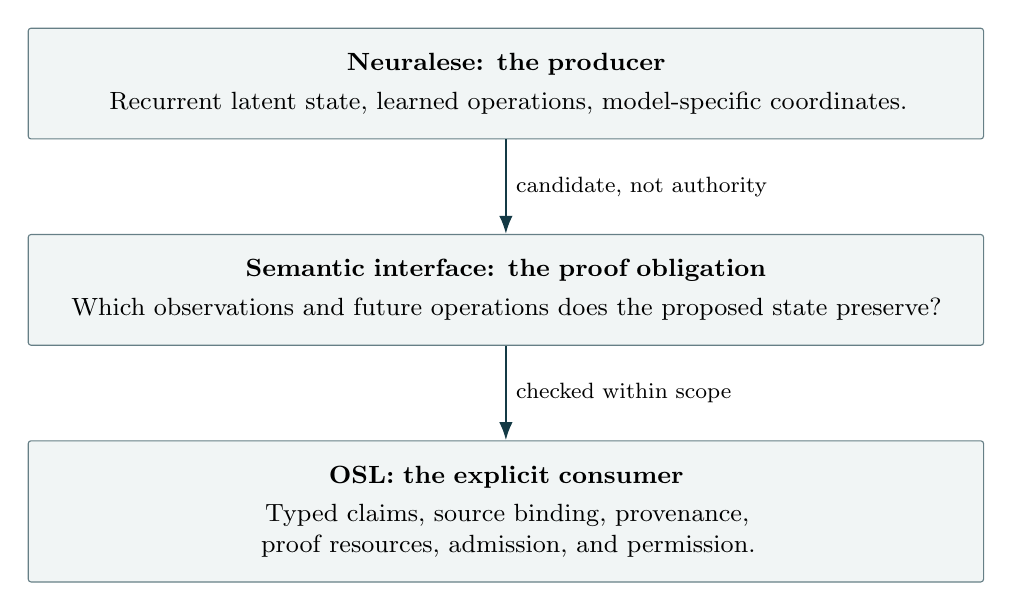
\begin{tikzpicture}[node distance=12mm]
\node[box,text width=11.5cm] (n) {\textbf{Neuralese: the producer}\\[3pt] Recurrent latent state, learned operations, model-specific coordinates.};
\node[box,text width=11.5cm,below=of n] (i) {\textbf{Semantic interface: the proof obligation}\\[3pt] Which observations and future operations does the proposed state preserve?};
\node[box,text width=11.5cm,below=of i] (o) {\textbf{OSL: the explicit consumer}\\[3pt] Typed claims, source binding, provenance, proof resources, admission, and permission.};
\draw[arr] (n)-- node[right,font=\footnotesize]{candidate, not authority} (i);
\draw[arr] (i)-- node[right,font=\footnotesize]{checked within scope} (o);
\end{tikzpicture}
\end{center}
\textbf{What exists now.} OSL-Core 0.5 is executable and has freshly replayed finite evidence. Neuralese contains learned finite operator results and their retained failures. The interface in this edition uses a complete, supplied finite transition table. Its checker is exact for that model.

\textbf{What remains a research obligation.} A learned producer must yield a representation that the interface can interpret without borrowing the answer from an unrestricted translator. Checking a supplied table does not establish that a neural network implements the same table.

\begin{scopebox}
\textbf{The connection is operational, not rhetorical.} A source is accepted because stated equations or predicates pass, not because its description calls it ``machine-native.'' The same system can accept one scope and retain another as unresolved.
\end{scopebox}
\textit{Read next:} OSL manuscript, Sections 1--3 and the semantic-checkpoint section; Neuralese manuscript, Sections 1--3. The proof-carrying and causal-abstraction background is cited in those papers.
\clearpage

\section*{2\quad A checkpoint that really preserves future computation}
The new finite demonstrator has concrete states $(a,b,u)$: eight visible D4 states $(a,b)$ and a private bit $u$. It exposes sixteen concrete states but only eight semantic classes.
\begin{center}
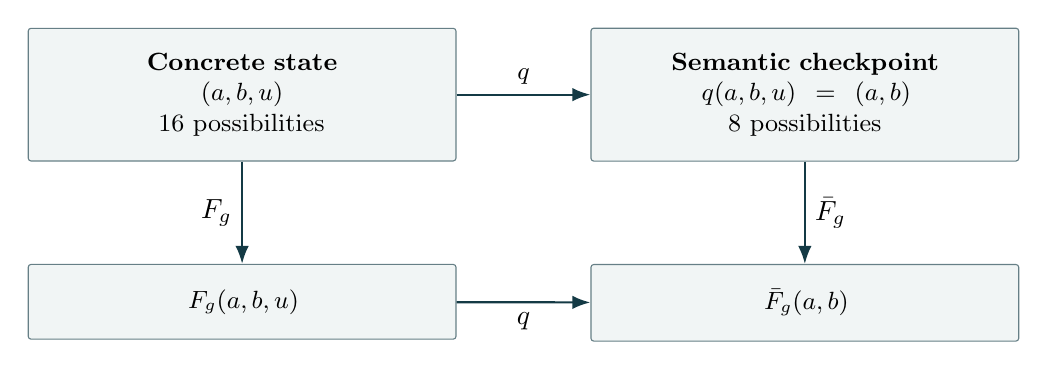
\begin{tikzpicture}[node distance=13mm]
\node[box,text width=4.8cm] (x) {\textbf{Concrete state}\\$(a,b,u)$\\16 possibilities};
\node[box,text width=4.8cm,right=17mm of x] (q) {\textbf{Semantic checkpoint}\\$q(a,b,u)=(a,b)$\\8 possibilities};
\draw[arr] (x)--node[above,font=\small]{$q$}(q);
\node[box,text width=4.8cm,below=of x] (fx) {$F_g(a,b,u)$};
\node[box,text width=4.8cm,below=of q] (fq) {$\bar F_g(a,b)$};
\draw[arr] (x)--node[left]{$F_g$}(fx);
\draw[arr] (q)--node[right]{$\bar F_g$}(fq);
\draw[arr] (fx)--node[below]{$q$}(fq);
\end{tikzpicture}
\end{center}
The square must commute at \emph{every declared state}:
\[
 q(F_g(s))=\bar F_g(q(s)),\qquad O(s)=\bar O(q(s)).
\]
The operations are
\[
 r(a,b,u)=(a+1,b,u),\quad f(a,b,u)=(-a,1-b,u),\quad v(a,b,u)=(a,b,1-u).
\]
Since none of them makes the private bit visible, the checkpoint may discard it. The checker tests all states and generators. Induction then gives preservation for all finite operation words of this declared machine, not just a test-depth panel.

\begin{scopebox}
\textbf{Checkpoint size is justified by future use.} Losing $u$ is permitted for this observation interface. Adding a new operation that copies $u$ into the visible state would invalidate the old scope and require a new certificate.
\end{scopebox}
The implementation is in \path{interface/semantic_interface.py}. It serializes the semantic class together with source, certificate, and scope digests. Those digests bind content; they do not authenticate a person or prove that the state arose in a particular historical episode.
\clearpage

\section*{3\quad Today's answer is not tomorrow's state}
Consider a two-bit machine. Its current output is the first bit. Its next operation swaps the bits.
\begin{center}
\begin{tabular}{ccccc}
\toprule Concrete state & Output now & State after swap & Output then & Same present class?\\\midrule
$(0,0)$ & 0 & $(0,0)$ & 0 & Yes, with $(0,1)$\\
$(0,1)$ & 0 & $(1,0)$ & 1 & But future differs\\
$(1,0)$ & 1 & $(0,1)$ & 0 & Yes, with $(1,1)$\\
$(1,1)$ & 1 & $(1,1)$ & 1 & But future differs\\\bottomrule
\end{tabular}
\end{center}
\textbf{Present-only compression:} retain one bit. There are two output classes.

\textbf{Continuation-preserving compression:} retain both bits. There are four classes because the next swap can reveal the discarded bit.

This is why a state that predicts an answer is not automatically a valid recurrent workspace. Neuralese needs both a history budget and a future-observation budget:
\[
 Q_{L,H}=R_{\le L}/\!\sim_H.
\]
$L$ says which states can have been reached. $H$ says how many further operations can be used to distinguish them. These are independent axes.

\begin{center}
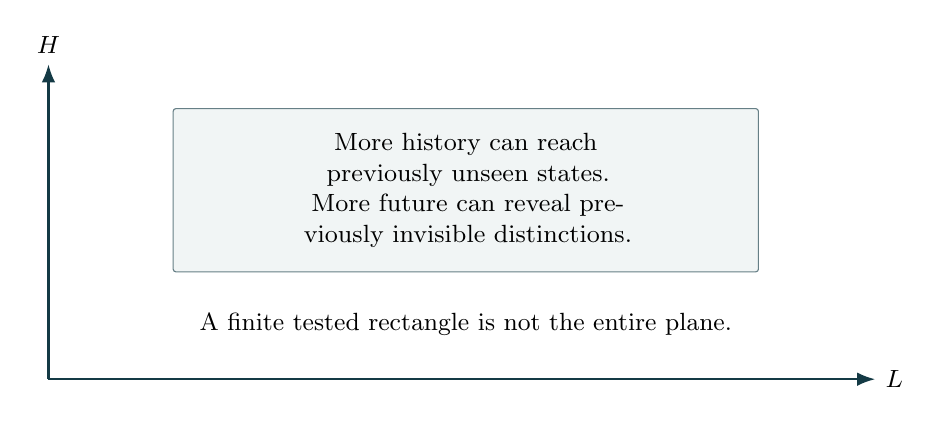
\begin{tikzpicture}
\draw[arr] (0,0)--(10.5,0) node[right,font=\small]{$L$};
\draw[arr] (0,0)--(0,4.0) node[above,font=\small]{$H$};
\node[box,text width=6.8cm] at (5.3,2.4) {More history can reach previously unseen states.\\More future can reveal previously invisible distinctions.};
\node[align=center,font=\small] at (5.3,.7) {A finite tested rectangle is not the entire plane.};
\end{tikzpicture}
\end{center}
The Neuralese completion-surface audit is organized around exactly this distinction. Many correct ordinary-history decisions coexist with delayed failures after longer paths. The figure is a definition diagram, not a measured heat map.
\clearpage

\section*{4\quad Numerical stability and semantic stability are different}
A rotation preserves norm perfectly. It can still move a state into the wrong decision region.
\begin{center}
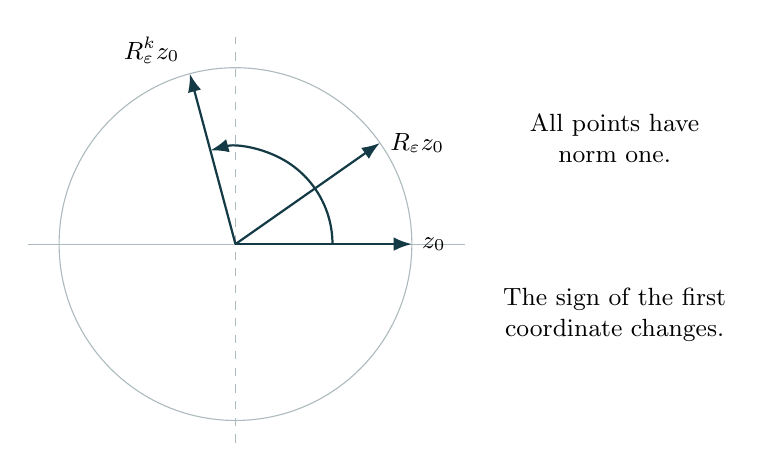
\begin{tikzpicture}[scale=1.12]
\draw[ink!35] (0,0) circle (2);
\draw[ink!35] (-2.35,0)--(2.6,0);
\draw[ink!35,dashed] (0,-2.25)--(0,2.35);
\draw[arr] (0,0)--(2,0) node[right,font=\small]{$z_0$};
\draw[arr] (0,0)--({2*cos(35)},{2*sin(35)}) node[right,font=\small]{$R_\varepsilon z_0$};
\draw[arr] (0,0)--({2*cos(105)},{2*sin(105)}) node[above left,font=\small]{$R_\varepsilon^k z_0$};
\draw[arr] (1.1,0) arc (0:105:1.1);
\node[align=center,font=\small] at (4.3,1.2) {All points have\\norm one.};
\node[align=center,font=\small] at (4.3,-.8) {The sign of the first\\coordinate changes.};
\end{tikzpicture}
\end{center}
In the explicit counterexample, the intended semantic action is the identity but the implementation is $R_\varepsilon$. Repetition accumulates an angular error $k\varepsilon$. A margin-based readout eventually changes class even though overflow, underflow, and norm explosion never occur.

\begin{scopebox}
\textbf{What the later operator study contributes.} It supplies an empirical counterpart to the distinction, not proof that every failure is a rotation. The hard-isometry architecture controls norm by construction; the overall learned-semantic gate conjunction still fails.
\end{scopebox}
For normalized linear dynamics,
\[
 F_M(z)=\frac{Mz}{\|Mz\|},\qquad
 DF_M(z)=\frac{(I-uu^{\mathsf T})M}{\|Mz\|}.
\]
The radial scale is removed, but the angular derivative need not contract. A claim about a stable semantic fiber must identify that fiber; a full-tangent derivative cannot silently substitute for it.
\clearpage

\section*{5\quad Read each result at its actual level}
\begin{center}
\begin{tabularx}{\textwidth}{>{\RaggedRight\arraybackslash}p{.25\textwidth}>{\RaggedRight\arraybackslash}X}
\toprule Record & What it supports, and what it does not\\\midrule
OSL-Core 0.5 & 168 fresh tests; corpus 66/66; 1,825 reproduced receipts. This is finite executable evidence, not universal interpreter soundness.\\
Stable Quotient & Strong two-seed structured-family and intervention results through tested depths. Arbitrary-family and longer-path limitations remain.\\
Operator Workspace & Completed 48-cell study. Eight of 26 primary gates pass. Norm preservation is not overall semantic success.\\
Completion Surface & More than 33 million correct ordinary-history continuation decisions. The registered cumulative and path-flatness failures remain.\\
Packet Closure & Training/execution complete, but assay A15 fails. The full developmental claim is not evaluated.\\
Invariant Kernel & Calibration stop. Untouched screen and pilot were not run.\\
Semantic Retraction & Armed, unspent, capacity-gated. 84 checkpoint-free tests are machinery checks, not learned results.\\
G1 pilot & Engineering passes, scientific conjunction fails. Shuffling retained the same IID accuracy.\\\bottomrule
\end{tabularx}
\end{center}
\textbf{Three questions must stay separate.}

Did the code run? Did the assay measure the intended quantity? Did the substantive hypothesis pass its preregistered gates? A positive answer to the first is not a shortcut past the other two.

\textbf{Fresh versus retained.} This edition reruns bounded code and record checks. It does not retrain the historical neural models or declare their results independently replicated. The named archives preserve the original positive results, failures, and stop rules.

\textit{Source map:} OSL manuscript's verification section; Neuralese manuscript's lineage and experimental sections; \path{SOURCE_LEDGER.json}; each project's \path{validation/} directory.
\clearpage

\section*{6\quad Admission is a transition with an obligation}
The new demonstrator sends a finite checkpoint through the actual OSL-Core 0.5 runtime. Its two paths deliberately end differently.
\begin{center}
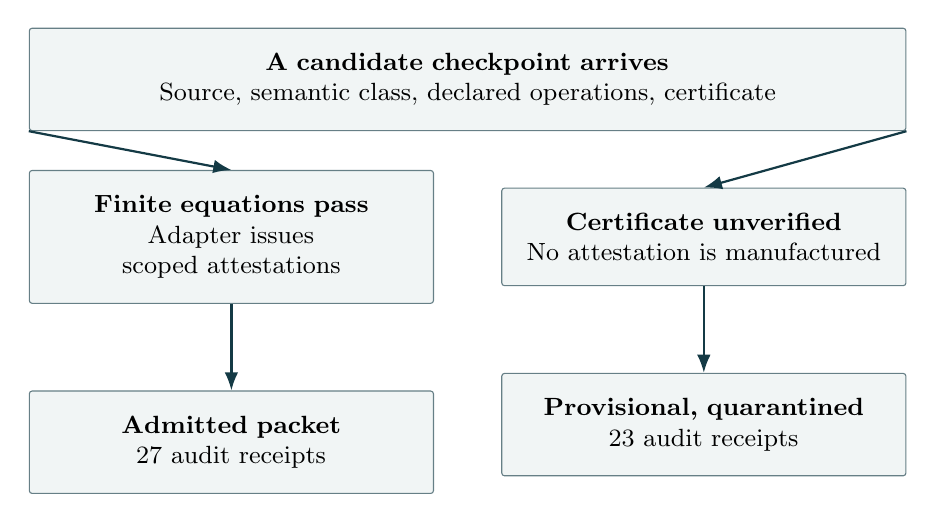
\begin{tikzpicture}[node distance=11mm]
\node[box,text width=10.5cm] (proposal) {\textbf{A candidate checkpoint arrives}\\Source, semantic class, declared operations, certificate};
\node[box,text width=4.5cm,at={(-3,-2)}] (pass) {\textbf{Finite equations pass}\\Adapter issues scoped attestations};
\node[box,text width=4.5cm,at={(3,-2)}] (fail) {\textbf{Certificate unverified}\\No attestation is manufactured};
\node[box,text width=4.5cm,below=of pass] (admit) {\textbf{Admitted packet}\\27 audit receipts};
\node[box,text width=4.5cm,below=of fail] (quarantine) {\textbf{Provisional, quarantined}\\23 audit receipts};
\draw[arr] (proposal.south west)--(pass.north);
\draw[arr] (proposal.south east)--(fail.north);
\draw[arr] (pass)--(admit);\draw[arr] (fail)--(quarantine);
\end{tikzpicture}
\end{center}
Both paths pass the base receipt checker and the domain semantic checker. The quarantined path is a correct outcome, not a broken demonstration. Neither path invokes an external tool or performs a real-world action.

\begin{scopebox}
\textbf{Provenance is not truth.} An intact record can faithfully preserve a false input. A certificate can establish equations for a supplied finite model without proving that a learned model or the physical world realizes it. A digest commits to bytes, not to a principal's identity.
\end{scopebox}
Similarly, communicating B's observation to A can justify A's use of communicated evidence without making it a firsthand observation by A. The distinction is represented in OSL's memory and provenance rules. A thousand copies of one observation should not become a thousand independent observations merely by passing through more agents.

\textit{Executable entry:} \path{interface/run_demo.py}. The generated source, traces, final states, and checker outcomes are preserved under \path{interface/examples/}.
\clearpage

\section*{7\quad Reproduce the edition without consuming new experiments}
From the complete package root:
\begin{lstlisting}[language=bash]
python verify_release.py
python run_current_checks.py
python interface/run_demo.py --output ../local_demo
python build_manuscripts.py --output ../rebuilt_papers
\end{lstlisting}
\textbf{Manifest verification} checks the packaged bytes and recursive source-archive integrity. It is not a scientific efficacy certificate.

\textbf{Current checks} run the fresh finite interface, OSL-Core tests, corpus replay, and bounded Discovery Bridge checks in temporary working copies. Reports are written outside the sealed source tree. The Core 0.5 copy uses its original release directory name because its own manifest binds that name.

\textbf{Manuscript rebuild} requires a TeX distribution with the packages listed in the source. It writes to a separate destination and does not silently reseal the edition.

\begin{scopebox}
\textbf{Do not run every discovered script indiscriminately.} The Semantic Retraction learned bank is unspent, the Entry--Cone learned endpoint is one-shot, and the invariant-kernel branch has a calibration stop. These rules remain in force. No default command in this edition opens a new learned bank, trains a model, or downloads a checkpoint.
\end{scopebox}
\textbf{Reading order.} Start with the two new manuscripts. Consult the original 88-page OSL monograph for the broader historical mathematical development. Use the source ledger to select a Neuralese branch and its current results document before running its own commands. Source packages have separate environments and are not flattened into a fictional common neural runtime.

\textbf{What finalization means here.} The manuscripts, reference programs, reading map, claim status, and recoverable evidence are fixed together. The open learning and mechanization problems are stated rather than renamed. No Lean verification or general learned Neuralese-to-OSL translation is claimed.

\vfill
\rule{\textwidth}{.4pt}
{\small Companion documents: \emph{OSL: Operator-Symbolic Language and Proof-Carrying Interfaces}; \emph{Neuralese: Recurrent Latent Operators, Causal Semantics, and Stability}. Research edition 1.0, Komorebi P., 6 October 2026. The full scholarly bibliography and version-bound internal references are in the manuscripts.}
\end{document}
